\documentclass[11pt]{article}
\usepackage{amsmath,amssymb,amsbsy,amsgen,amsopn,amsthm}
\usepackage{mathrsfs}
\usepackage{multirow,booktabs}
\usepackage{threeparttable}
\usepackage{hyperref}
\usepackage{times}
\usepackage[margin=1in]{geometry}


\renewcommand{\baselinestretch}{1.03}

\newtheorem{theorem}{Theorem}
\newtheorem{lemma}{Lemma}
\newtheorem{corollary}{Corollary}
\newtheorem{definition}{Definition}
\newcommand{\Qset}{\mathbb{Q}}
\newcommand{\Rset}{\mathbb{R}}
\newcommand{\Zset}{\mathbb{Z}}
\newcommand{\Nset}{\mathbb{N}}
\newcommand{\Mfam}{\mathcal{M}}
\newcommand{\Afam}{\mathcal{A}}
\newcommand{\Cfam}{\mathcal{C}}
\newcommand{\Ffam}{\mathcal{F}}
\newcommand{\Vfam}{\mathcal{V}}
\newcommand{\Lfam}{\mathcal{L}}
\newcommand{\Bfam}{\mathcal{B}}
\newcommand{\Pfam}{\mathcal{P}}
\newcommand{\OPT}{{\rm OPT}}
\newcommand{\LP}{{\tt PCLP}}
\newcommand{\NPCLP}{{\tt NPCLP}}
\newcommand{\CoreLP}{{\tt SimpleLP}}
\newcommand{\CoreDual}{{\tt SimpleDual}}
\newcommand{\true}{\mbox{true}}
\newcommand{\false}{\mbox{false}}

\usepackage[linesnumbered,boxed]{algorithm2e}
\setlength{\algomargin}{1.5em}

\usepackage{tikz}
\usetikzlibrary{backgrounds}
\usetikzlibrary{snakes}
\usetikzlibrary{shapes}
\usetikzlibrary{trees}  
\tikzstyle{vertex}=[circle,draw, inner sep=2.3pt]
\tikzstyle{terminal}=[circle,draw,fill, inner sep=2.3pt]
\tikzstyle{biset}=[fill=gray,fill opacity=.2, line width=8pt, draw=gray]
\tikzstyle{biset outer}=[dotted,line width=2pt]

\title{Spider covers for prize-collecting network activation problem}

\author{Takuro Fukunaga\footnote{National Institute of Informatics,
2-1-2 Hitotsubashi, Chiyoda-ku, Tokyo, Japan.
JST, ERATO, Kawarabayashi Large Graph Project, Japan.
Email: takuro@nii.ac.jp}}

\date{}

\begin{document}
\maketitle
\begin{abstract}
In network activation problem, each edge in a graph is associated with an
 activation function that decides 
 whether the edge is activated from weights assigned
 to its end nodes.
 The feasible solutions of the problem are node weights such that the
 activated edges form graphs of required connectivity,
 and the objective is to find a feasible solution minimizing its total
 weight.
 In this paper, we consider a prize-collecting version of the network
 activation problem and present the first nontrivial approximation algorithms.
 Our algorithms are based on a new linear programming relaxation of the problem.
 They round optimal solutions for the relaxation by repeatedly computing
 node weights
 activating subgraphs, called spiders, which are known to be useful for
 approximating the network activation problem.
 For the problem with node-connectivity requirements, we also present a new
 potential function on uncrossable biset families
 and use it to analyze our algorithms.
\end{abstract}

\section{Introduction}
\subsection{Problem}
{\em Network activation problem}
is a problem of 
activating a well-connected network by assigning weights to
nodes.
The problem is formally described as follows. Given a graph  and
a set  of non-negative real numbers such that  and
 for any ,
a solution in the problem is a
node weight function .
For ,
let  and  
denote the unordered and ordered pairs of  and , respectively.
Each edge  is associated with an activation function  such that
 holds for any .
In this paper, each activation function  is supposed to be
{\em monotone}, i.e.,
if  for some ,
then  for any  with  and .
An edge  is \emph{activated} by  if
.
Let  be the set of edges activated by  in .
A node weight function  is feasible 
in the network activation problem
if  satisfies given constraints, and the objective of the problem is to find a feasible
node weight function  that minimizes , denoted by
. 
We assume throughout the paper that  is undirected even though
the problem can be defined for directed graphs as well.

In this paper, we pose connectivity constraints 
on the set  of activated edges.
Namely, we are given
demand pairs  associated with
connectivity requirements  defined as natural numbers.
 denotes ,  denotes ,
and a node that participates in some demand pair is called a {\em terminal}.
The constraints require that
the connectivity between  and  in
the graph  is at least  for each .
We consider three definitions of the connectivity:
edge-connectivity, node-connectivity, and element-connectivity.
The edge-connectivity between two nodes  and  is the maximum
number of edge-disjoint paths between  and ,
and the node-connectivity 
between  and  is the maximum
number of inner disjoint paths between  and .
The element-connectivity is defined only for pairs of terminals,
and for two terminals  and , it is defined as the maximum number
of paths between them that are disjoint in edges and in non-terminal nodes.
The edge-connectivity network activation problem denotes the problem with the edge-connectivity
constraints.
The node- and the element-connectivity network activation problems 
are defined similarly.

The network activation problem is closely related to
the \emph{survivable network design problem} (SNDP),
a problem of constructing a cheap network that is sufficiently connected.
A feasible solution to the SNDP is a subgraph  of a given graph 
that satisfies the connectivity constraints.
There are two popular variations, called the edge- and
node-weighted SNDPs.
In the edge-weighted SNDP, each edge in the graph is associated with a
weight , and the objective is to minimize the weight  of  defined as
.
In the node-weighted SNDP, 
a weight  is given for each node , and the objective is
to minimize , where  denotes the set of
end nodes of edges in .
We denote  by  in the sequel.
It is known that the node-weighted SNDP generalizes the edge-weighted
SNDP.

It can be seen that the network activation problem extends the node-weighted SNDP.
Given node weights ,
let ,
and define a monotone activation function  for  so that
 if and only if  and .
A minimal solution  to the network activation
problem with these activation functions
does not assign a weight larger than  to .
Hence, if an edge activated by  is incident to a node , 
then  holds without loss of generality.
Therefore, the node-weighted SNDP with  is equivalent to the network activation problem
with  defined from .

The extension from the SNDP to the network activation problem is not
only important from a technical viewpoint but also for practical
reasons. In the node-weighted SNDP, for each node, one is required to decide whether it
is chosen.  In contrast, the network activation problem demands
a decision concerning which weight is assigned to a node. In other words, the
network activation problem admits more than two choices while the
node-weighted SNDP admits only two choices for each node.  This rich
structure of the network activation problem enables to capture many
problems motivated by realistic applications.  In fact,
Panigrahi~\cite{Panigrahi11wireless} discussed numerous applications to
wireless networks.  In wireless networks, the success of communication
between two base stations depends on factors such as physical
obstacles between them, positions of antennas, and signal strength.
Panigrahi suggested that many problems related to wireless networks can
be modeled by the network activation problem.

Our main contribution in this paper is to develop algorithms for 
a prize-collecting version of the network activation
problem, which we call the {\em prize-collecting network activation
problem} (PCNAP). 
In the PCNAP,
each demand pair  is associated with not only a
connectivity requirement , but also a non-negative real number
, which is called the \emph{penalty}.
The edge set  activated by a solution  
is allowed to violate the
connectivity requirements,
but it has to pay the penalty  if it does not satisfy the connectivity
requirement for . 
The objective of the PCNAP
is to minimize the sum of 
 and the penalties we have to pay.

We also consider two variations of the PCNAP.
The {\em rooted node-connectivity PCNAP} is a special case of the
node-connectivity PCNAP such that 
a root node  is specified and the demand pairs
are .
In the {\em subset node-connectivity PCNAP},
terminals  
and penalties  are given instead of demand pairs.
Let  be the set of activated edges. 
In addition to node-weights,
a solution chooses  such that 
every pair of terminals  and  
with 
is -connected in the graph .
The penalty is .
We note that the subset node-connectivity PCNAP is not a special case of
the node-connectivity PCNAP because the above setting cannot be represented by 
connectivity demands and penalties on terminal pairs.


In all of the known applications, it is reasonable to assume 
.
In fact, all previous research~\cite{Nutov13activation,Panigrahi11wireless} studied the network activation problem 
under this assumption.
In this paper, we proceed on the same assumption and 
design algorithms
that run in polynomial time of  and the size of .

\subsection{Related work} 

The SNDP is a well-studied optimization
problem, and there are substantial number of studies regarding algorithms for
it. The best known approximation factors for the edge-weighted SNDP are two
for the edge-~\cite{Jain01} and element-connectivity~\cite{FleischerJW06},
and  for node-connectivity~\cite{ChuzhoyK12}. 
For the node-weighted SNDP, 
Nutov~\cite {Nutov10node-weights} gave an -approximation algorithm with edge-connectivity requirements, and
element-connectivity requirements in~\cite{Nutov12uncrossable}. His algorithm
is based on an algorithm for the problem of covering uncrossable biset
families by edges, where a biset is an ordered pair of two node sets, and an uncrossable family 
is a family closed under some uncrossing operations (we will present their formal definitions later). 
However, his analysis of the
algorithm for covering uncrossable biset families has an error.
We will explain it in Section~\ref{sec.potential}.

The prize-collecting SNDP has also been well studied.
As for edge-weighted graphs,
we refer to only Hajiaghayi et al.~\cite{HajiaghayiKKN12} 
whereas many papers studied related problems such as the prize-collecting Steiner tree and forest.
Recently much attention has been paid to node-weighted graphs.
K\"onemann, Sadeghian, and Sanit\`a~\cite{Konemann13CoRR} gave an -approximation algorithm for the prize-collecting node-weighted Steiner tree problem.
Their algorithm has the Lagrangian multiplier preserving property, which is
useful in many contexts.
They also pointed out a technical error in Moss and Rabani~\cite{MossR07}.
Bateni, Hajiaghayi, and Liaghat~\cite{BateniHL13} gave an -approximation algorithm for the prize-collecting node-weighted Steiner forest
problem with application to the budgeted Steiner tree problem.
Chekuri, Ene, and Vakilian~\cite{ChekuriEV12} gave an -approximation for the prize-collecting SNDP with edge-connectivity
requirements, which they later improved to -approximation
and also extended to 
the element-connectivity
requirements (refer to \cite{Vakilian13}).
We note that the proof in~\cite{Vakilian13} implies that the 
algorithm in~\cite{Nutov12uncrossable} works for the node-weighted SNDP
with element-connectivity requirements,
as Nutov originally claimed, even though his analysis of the algorithm for covering
uncrossable biset families is not correct in general.
We also note that 
the algorithm for the element-connectivity requirements in~\cite{Vakilian13} implies 
-approximation for node-connectivity requirements,
using the reduction from node-connectivity requirements to 
the element-connectivity requirements presented by Chuzhoy and Khanna~\cite{ChuzhoyK12}.

Concerning the network activation problem, 
Panigrahi~\cite{Panigrahi11wireless} gave -approximation
algorithms for  and proved
that it is NP-hard to obtain an -approximation algorithm even
when activated edges are required to be a spanning tree.
Nutov~\cite{Nutov13activation} presented approximation algorithms for
higher connectivity requirements, including -approximation for
the edge- and element-connectivity and -approximation for
the node-connectivity.
He also discussed special node-connectivity requirements such as rooted and
subset requirements.
These results are built based on his research in~\cite{Nutov12uncrossable} for
covering uncrossable biset families. 
This contains an error as
mentioned above, and 
the rectification offered in~\cite{Vakilian13} cannot be extended to the network
activation problem.
Therefore, the network activation problem currently
has no non-trivial algorithms for the element- and node-connectivity.
One contribution of this paper is to rectify the Nutov's error and to provide
algorithms for these problems.


An important factor
in most of the research mentioned above is the {\em greedy spider cover algorithm}.
The notion of {\em spiders} was invented by Klein and Ravi~\cite{KleinR95} in
order to solve
the node-weighted Steiner tree problem. 
It was originally defined as a tree that admits at most one
node of degree larger than two and that spans at least two terminals.
The node of degree larger than two is called the {\em head}, 
and nodes of degree one are called the {\em feet}
of the spider. 
It is supposed without loss of generality that each foot of a spider is a terminal.
If all nodes have degrees of at most two, then an arbitrary node is chosen to be the head.
Klein and Ravi~\cite{KleinR95} proved that any Steiner tree can be
decomposed into node-disjoint spiders so that each terminal is included by
some spider. The {\em density} of a subgraph is defined as 
its node weight divided by the number of terminals included by it.
The decomposition theorem implies that there exists a spider with a
density of at
most that of Steiner trees. 
Since contracting a spider with  feet decreases the number of
terminals by at least ,
a greedy algorithm to 
repeatedly contract minimum density spiders
achieves -approximation.
Minimum density spiders are hard to compute but their relaxations can be
computed by a simple algorithm that involves first guessing the place of the head and 
number of feet, which is possible
because there are only  options for each. Let  be the head, and
 be the number of feet.
We then compute a shortest path from  to each terminal, and
choose the  shortest paths from them.
The union of these shortest paths is not necessarily a spider, but its
density is at most that of spiders, and contracting the union can play the
same role as contracting spiders.
Nutov~\cite{Nutov10node-weights,Nutov12uncrossable,Nutov13activation}
extended the notion of spiders to uncrossable biset families, and demonstrated in the
sequence of his research that they are useful for the node-weighted SNDP and the
network activation problem.  


\subsection{Our results}

The main result in this paper is to present approximation algorithms for
the PCNAP.
Our algorithms achieve -approximation for the
edge-connectivity PCNAP, and
-approximation for the element-connectivity PCNAP.
Table~\ref{table.results} summarizes the approximation factors achieved by our algorithms
and previous studies.
Using decompositions of connectivity requirements given in 
\cite{ChuzhoyK12,Nutov12uncrossable,Nutov12subset},
we can also achieve approximation factors
 for the node-connectivity PCNAP
and  for the rooted and
subset node-connectivity PCNAPs.
Our results 
give the first non-trivial algorithms for the PCNAP.
We also recall that, 
besides our algorithms,
no algorithms are known
even for the element- and node-connectivity network activation problems
because the analysis of the algorithms claimed 
by Nutov~\cite{Nutov12uncrossable,Nutov13activation}
contains an error.
For wireless networks, it is natural to consider node-connectivity, 
which represents tolerance against node failures,
rather than edge-connectivity, which represents tolerance against link
failures.
Hence, our results are important for not only theory but also applications.


\begin{table*}
\centering
\caption{Approximation factors for the edge-weighted SNDP, node-weighted SNDP, and 
the network activation problem}
\label{table.results}

\begin{threeparttable}
\begin{tabular}{lllll}
\toprule
 & \multicolumn{2}{l}{non-prize-collecting} & \multicolumn{2}{l}{prize-collecting}\\
\midrule
{\bf edge-connectivity}&&&&\\
edge-weighted SNDP & 2 & Jain~\cite{Jain01} & 2.54 & Hajiaghayi et al.~\cite{HajiaghayiKKN12} \\
node-weighted SNDP & 
	 & Nutov~\cite{Nutov10node-weights} 
	&  & Chekuri et al.~\cite{ChekuriEV12}\\
network activation & 
	 & Nutov~\cite{Nutov13activation}
	&  & [this paper]\\
\midrule
{\bf element-connectivity}&&&&\\
edge-weighted SNDP
	& 2 & Fleischer et al.~\cite{FleischerJW06}
	& 2.54 &Hajiaghayi et al.~\cite{HajiaghayiKKN12}\\
node-weighted SNDP
	&  & Vakilian \cite{Vakilian13}\tnote{1}
	&  & Vakilian \cite{Vakilian13}\\
network activation  
 &  & [this paper]\tnote{1}
 &  & [this paper]\\
\bottomrule
\end{tabular}
\begin{tablenotes}\footnotesize
\item[1] Nutov~\cite{Nutov12uncrossable,Nutov13activation} claimed -approximation
algorithms for the node-weighted SNDP and the network activation problem with element-connectivity 
constraints, but these contained an error.
\end{tablenotes}
\end{threeparttable}
\end{table*}



Let us present a high level overview of our algorithms.
Our algorithms first reduce the problem with high connectivity requirements
to the \emph{augmentation problem},
which asks to increase the connectivity of demand pairs by one.
This is a standard trick for SNDP,
and we will show in Section~\ref{sec.preliminaries} that this trick can work
even for the PCNAP.
Then, our algorithms compute an optimal solution to an LP relaxation, and 
discards some of the demand pairs according to the optimal solution, 
which is a popular way to deal with prize-collecting problems
since Bienstock~et~al.~\cite{BienstockGSW93}.
In the last step, the algorithms solves the problem using the greedy spider cover algorithm.
To obtain an approximation guarantee, we are required to show that 
the minimum density of spiders can be bounded
in terms of the optimal value of the LP relaxation.
We achieve this by presenting a primal-dual algorithm for computing spiders,
which is the same approach as~\cite{ChekuriEV12,BateniHL13,Vakilian13}.

As observed from this overview,
our algorithms rely on many ideas
given in the previous studies on the prize-collecting
SNDP and the network activation problem.
However, it is highly nontrivial to apply these ideas for the PCNAP, and 
we required several new ideas to obtain our algorithms.
Specifically,
the technical contributions of the present paper are the following three new findings:
an LP relaxation of the problem,
a primal-dual algorithm for computing spiders, and a 
potential
function for analyzing the greedy spider cover algorithm.
Below we explain these one by one.


\subsubsection*{LP relaxation}
Nutov's spider decomposition theorem is useful for 
the biset covering problem defined from the
SNDP and the network activation problem, but 
we have to strengthen it for solving their prize-collecting versions. 
We define an LP relaxation of the problem
and compare the minimum density of spiders with the density of
fractional solutions feasible to this relaxation. The same attempt has
been made previously by
\cite{BateniHL13,ChekuriEV12,Konemann13CoRR} for the node-weighted SNDP,
but our situation is much more complicated.
Each connectivity requirement in the node-weighted SNDP can be simply represented 
by demands on the number of chosen nodes in node cuts of graphs,
which naturally formulates an LP relaxation that performs well.
On the other hand,
the network
activation problem requires to decide which edges are
activated for covering bisets in addition to the decision on which weights are assigned to nodes
for activating the edges.
Hence an LP relaxation for the network activation problem needs
variables corresponding to edges and nodes whereas that for the node-weighted SNDP 
needs only variables corresponding to nodes.
However, 
dealing with both edge and node variables introduces 
a large integrality gap into
a natural LP relaxation for the network
activation problem, as we will see in Section~\ref{sec.LP}.
Hence we require to formulate an LP relaxation carefully.

In the present paper, 
we propose a new LP that lifts the natural LP relaxation for the PCNAP.
It is non-trivial even to see that our LP relaxes the PCNAP.
We prove it
using the structure of uncrossable biset families, wherein
any uncrossable biset family
can be decomposed into 
a polynomial number of ring biset families,
and 
the degree of each node is at most two in
any minimal edge cover of a ring biset family.
In addition,
the main result in this paper implies that
our LP has small integrality gap.

Let us mention that
the idea on formulating our LP relaxation is potentially useful for other covering problems.
The author pointed out
in his recent work~\cite{Fukunaga14}
that
a natural LP relaxation has a large integrality gap for many covering problems
in node-weighted graphs. He also presented several tight approximation algorithms
using the LP relaxations designed based on the idea we propose in the present paper.


\subsubsection*{Primal-dual algorithm for computing spiders}
For bounding the minimum density of spiders in terms of optimal
values of our relaxation, we will present a primal-dual algorithm for computing
spiders. 
Usually, a primal-dual algorithm computes fractional solutions feasible to
the dual of an LP relaxation together with primal solutions, but this seems
difficult for our relaxation because of its complicated form.
Hence, our algorithm does not directly
compute solutions feasible to the dual of our relaxation.
Instead, we define another LP simpler than our relaxation,
and our algorithm computes feasible solutions to the dual of this
simpler LP.
Although the simpler LP does not relax our relaxation, 
we can show that it is within a constant factor of our relaxation
if biset families are restricted to laminar families of cores, which are
bisets that do not include more than one minimal biset.
Our primal-dual algorithm 
computes dual solutions
that assign non-zero values only to variables corresponding to cores in 
laminar families.
Hence, the density of spiders can be analyzed in terms of our relaxation.

Summarizing, our algorithm uses two different LPs:
the LP based on the structure of uncrossable biset families
is used for deciding which demand pairs are discarded in the first step, and
the simpler LP 
with laminar core families is used
in the second step that iterates choosing spiders.
We note that the simpler LP cannot be used 
in the first step because of two reasons.
First,
we do not know beforehand which laminar core families will be used, and second, we have different laminar families in distinct iterations.

Although
our primal-dual algorithm for the simpler LP 
seems to be similar to primal-dual algorithms known for related
problems, 
its design and analysis is not trivial.
 One reason for this is the
existence of more than one choices of weights for each end node of activated edges as we have already
mentioned. Another reason is the involved structure of bisets. Since a biset is defined as an ordered pair of
two node sets, covering a biset family by edges is much more difficult problem than covering a set family,
for which primal-dual algorithms are often studied. Indeed, our algorithm utilizes many non-trivial
properties of uncrossable biset families.


\subsubsection*{Potential function for analyzing greedy spider cover algorithm}
Nutov~\cite{Nutov12uncrossable} claimed that
repeatedly choosing a constant approximation of minimum density spiders
achieves 
-approximation for covering uncrossable biset families.
This claim is true if biset families are defined from
edge-connectivity requirements.
However it is not true for all uncrossable biset families.
The claim is based on the fact that contracting a spider with  feet
decreases the number of minimal bisets by a constant fraction of .
However there is a case in which contracting a spider does not decrease
the number at all (see Section~\ref{sec.potential}).
Chekuri, Ene, and Vakilian~\cite{Vakilian13}
showed that the claim is true for biset families arising from the
node-weighted SNDP,
but it cannot be extended to arbitrary uncrossable biset families,
including those from the network activation problem.

To rectify this situation,
we will define a new potential function.
The new potential function depends on
the numbers of minimal bisets and
 nodes shared by more
than two minimal bisets.
If the number of minimal bisets does not decrease considerably when a
spider is selected, 
many new minimal bisets share the head of the spider.
This fact motivates the definition of the potential function.

With this new potential function,
the definition of density of an edge set will be changed to the total weight for
activating it divided by the value of the potential function.
We cannot prove that the minimum density of spiders is at most that of
biset family covers after changing the definition of density.
Instead, we will show that a spider minimizing the density in the old definition
approximates 
the density of biset family covers in the new definition within a factor of .
This proves that the greedy spider covering algorithm achieves
 -approximation for the biset
covering problem with uncrossable biset families.
Since Klein and Ravi~\cite{KleinR95},
the greedy spider cover algorithms have been applied to many problems
related to the node-weighted SNDP.
Considering this usefulness of the greedy spider cover algorithms,
our potential function is of independent interest
because it is required for analyzing the algorithms for
uncrossable biset families.

\subsection{Roadmap}
The remainder of this paper is organized as follows. 
Section~\ref{sec.preliminaries}
presents reduction from the PCNAP to the
augmentation problem
and introduces preliminary facts on biset families. 
Section~\ref{sec.LP}
defines our LP relaxation.
Section~\ref{sec.primal-dual} presents our primal-dual algorithm for
computing spiders, and Section~\ref{sec.potential}
presents a new potential function for analyzing the greedy spider covers.
Section~\ref{sec.algorithm} presents our algorithms, with
Section~\ref{sec.conclusion}
concluding this paper.

\section{Preliminaries}\label{sec.preliminaries}

\subsection{Reduction to the augmentation problem}\label{sec.augmentation}
First, we define the augmentation problem in detail.
We assume that there are two edge sets  and , and
activation functions are given for edges in .
The connectivity of each 
demand pair  is at least 
in the graph , 
and a subset  of  is feasible if
the connectivity of each demand pair in
 is at least .
The objective of the problem is to find a node weight function  so that  is feasible and
 is minimized.
In the prize-collecting augmentation problem, each demand pair

has a penalty , and if the connectivity of  is not
increased by , then we
must pay the penalty. The objective of the prize-collecting
augmentation problem is to find a node weight function  that
minimizes the sum of  and penalties of demand pairs of
connectivity smaller than  in .
PCNAP can be reduced to the
prize-collecting augmentation problem as follows.

\begin{theorem}\label{thm.augmentation}
 If the prize-collecting augmentation problem admits an
 -approximation algorithm, then PCNAP admits an -approximation algorithm.
\end{theorem}
\begin{proof}
 We sequentially define instances of the prize-collecting augmentation
 problem. In the first instance,
  is set to be empty and  is the edge set of the graph in the
 instance of the PCNAP. 
 Activation functions, demand pairs and their penalties are same as
 those in the PCNAP instance.
 The connectivity of each demand pair is  in ,
 and the requirement of a demand pair is satisfied 
 if its connectivity is increased to at least one in .
 
 We define the -th instance after solving the -th instance.
 Let  be the node weights computed by the
 -approximation algorithm for the -th instance,
 and  be the set of indices of demand pairs that are
 satisfied by  in the -th instance.
 We move the edges activated by  from  to .
 For each , the connectivity of   is at least
  in  after the update.
 Let .
 We define the demand pairs in the -th instance as ,
 .
 The activation functions in the -th instance 
 are same as those in the PCNAP instance.

 We repeat the above sequence until the -th instance is solved.
 Our solution to the PCNAP instance is .
 We prove that  achieves -approximation.
 Let  be an optimal solution for the PCNAP instance, and \{s_i,t_i\}E_{w^*}.
 Then,
 the optimal value of the PCNAP instance is 
 .
 If an edge is activated by  in the PCNAP instance,
 then it is either in  or is activated by  in the -th
 instance of the prize-collecting augmentation problem.
 Hence, a demand pair  with 
 is satisfied by  if it is satisfied by  in the PCNAP instance,
 implying that
 the objective value of  
 in the -th instance
 is at most .
 By the -approximability of ,
 we have

The objective value of  in the PCNAP instance is 

\end{proof}


\subsection{Biset covering problem}\label{sec.biset}
Here, we formulate the prize-collecting augmentation problem 
as a problem of activating edges covering bisets.
A {\em biset} is an ordered pair  of subsets of  such that . The former element of a biset is called the {\em inner-part} and the
letter is called the {\em outer-part}. 
We always let  denote the inner-part of
a biset  and  denote the outer-part of .
 is called the {\em boundary} of a biset  and is denoted
by .
For an edge set ,  denotes the set of edges in
 that have one end-node in  and the other in .
We say that an edge  {\em covers}  if 
, and a set  of edges {\em covers} 
a biset family  if each  is covered by some
edge in .



Let .
We say that a biset  {\em separates} a demand pair  if 
.
We define  as the family of bisets  such that
, , and  separates 
the demand pair .
According to Menger's theorem,  
increases the edge-connectivity of  in the augmentation problem
if and only if 
 covers .
We define  as the family of bisets  such that
 and  separates the demand pair .
 
increases the node-connectivity of  
if and only if 
 covers .
We define  as the family of bisets  such that
 for each .
 
increases the element-connectivity of  
if and only if 
 covers .

For two bisets  and , we define
, 
, 
and 
.
A biset family  is called {\em uncrossable}
if, for any , 
(i)~, or 
(ii)~ holds.
The following lemma indicates that the uncrossable biset families characterize
the augmentation problem with edge- and element-connectivity requirements.



\begin{lemma}\label{lem.edge-element}
For any ,
biset families
 and

are uncrossable.
\end{lemma}

Lemma~\ref{lem.edge-element} follows from the submodularity and
posimodularity of  and , and a simple case analysis.
The same claim can be found in
\cite{FleischerJW06,Nutov12uncrossable}, and we recommend referring to
them for the proof of Lemma~\ref{lem.edge-element}.


By Lemma~\ref{lem.edge-element},
the problem of finding a minimum weight edge set covering 
a given uncrossable biset family
contains the augmentation problem with edge- or element-connectivity
requirements. The biset family

defined from the node-connectivity requirements is not
necessarily uncrossable. However, it was shown previously in~\cite{ChuzhoyK12,Nutov12uncrossable,Nutov12subset}
that this family can be decomposed into uncrossable families, and the union of
covers of these uncrossable families gives a good approximate solution
for the node-connectivity augmentation problem.
We apply this approach for dealing with node-connectivity constraints
(see Section~\ref{sec.algorithm}).

We define the {\em biset covering problem}
as 
the problem of 
minimizing the sum of node weights under the constraint that the edges
activated by the node weights cover given biset families.
The prize-collecting version of the biset covering problem
is defined as follows.
Given an undirected graph  such that each edge in  is
associated with an activation function, 
demand pairs
 with penalties
,
and a biset family  on .
For , let  be the family of bisets in 
that separate .
We say that  is {\em violated} by an edge set 
if .
The penalty of  is  where the summation is
taken over all  such that  violates some biset in .
The objective of the problem is to find  that minimizes 
the sum of  and penalty of .
This problem generalizes
the prize-collecting augmentation problem,
and hence, it suffices to present an algorithm for this problem.

Our results require several properties of uncrossable biset families.
We say that bisets  and  are {\em strongly disjoint}
when both  and  hold.
When  and ,
we say .
Minimality and maximality in a biset family are defined with regard to
inclusion.
A biset family  is called {\em strongly laminar}
when, if  are not strongly disjoint, then 
they are comparable (i.e.,
 or ).
A minimal biset in a biset family  is called a {\em min-core}, and
 denotes the family of min-cores in .
A biset is called a {\em core} if it includes only one min-core, and 
 denotes the family of cores in ,
where min-cores are also cores.
When  is clear from the context, we may simply denote them
by  and .

For a biset family , biset , and node , 
 denotes 
and  denotes .
A biset family  is called a {\em ring-family}
if
 hold
for any .
A maximal biset in a ring-family is unique because ring-families are closed under union.


\begin{lemma}\label{lem.uncrossable}
If  is an uncrossable family of bisets, then the following properties hold\/{\rm :}
\begin{enumerate}
 \item[\rm (i)]  is a ring-family for any 
	      .
 \item[\rm (ii)] Let  be distinct min-cores.
	      For any  and , 
	      both 
	      and 
	      hold.
 \item[\rm (iii)] Let  be distinct min-cores.
	      Then  is strongly disjoint with
	      any .
	      In particular, min-cores are pairwise strongly disjoint.
\end{enumerate}
\end{lemma}

The proof of Lemma~\ref{lem.uncrossable} can be found
in~\cite{Nutov12uncrossable}. 

For a biset family  and an edge set , let .
The following lemma is required when we compute solutions recursively.

\begin{lemma}\label{lem.residual-uncrossable}
 Let  be a family of bisets and .
 Then  is
 uncrossable if  is uncrossable.
  is a ring-family if  is a ring-family.
\end{lemma}
\begin{proof}
If bisets  and  satisfy
,
then 
all , ,
, and 
are empty.
The claim follows from this fact.
\end{proof}


Below, we consider directed edges for technical reasons.
 denotes the set of directed edges obtained by orienting the edges
in  in both directions.
 denotes  for a biset .
We say that a directed edge  covers a biset  if ,
and a set  of directed edges covers a biset family  if each
biset in  is covered by some edge in .
The following lemma will be required to prove that our LP relaxes the
prize-collecting biset covering problem.

\begin{lemma}\label{lem.ring-cover}
 Let  be an inclusion-wise minimal set of directed edges 
 that covers a ring-family  of bisets.
 Then the in-degree and out-degree of each node in the graph  
 is at most one.
\end{lemma}
\begin{proof}
 Let .
 We see that at most one edge in  leaves .
 For arriving at a contradiction, suppose that
  contains two edges  and .
 By the minimality of ,
 there exist   
 with  and 
   
 with .
 Note that .
 We have 
 because  is a ring-family.
  and  hold,
 and hence  holds.
 However, this means that  contains
 an edge distinct from  and ,
 and that this edge covers  or .
 This contradicts the definition of  or .

 We can also see that
  contains at most one edge entering .
 To the contrary, suppose that
 there are two edges  and  in .
 There exist   
 with  and 
   
 with  by the minimality of
 .
 Note that .
 We have .
 If  covers ,
 then it covers  as well, which is a contradiction.
 Hence  does not cover .
 Similarly, we can see that  does not cover , which means that  contains
 an edge that is distinct from  and , and it
  covers  or .
 However, this contradicts the definition of  or .
\end{proof}


\section{LP relaxation for prize-collecting augmentation problem}
\label{sec.LP}

In this section, we present an LP relaxation for the prize-collecting
augmentation problem. 
Henceforth, we let  denote the target connectivity from now on; 
The connectivity of each demand pair is  in ,
and the problem
requires an increase in the connectivity of each demand pair by at least one.

For an edge ,
let  denote the set of pairs 
such that 
.
A natural integer programming (IP) formulation for the prize-collecting biset covering
problem can be given by preparing 
variables  for each  and , 
 for each  and , 
and  for each .
 indicates that  is activated 
by weights  with  and .
 is equal to 1 if  is assigned the weight , and  otherwise.
 indicates whether the connectivity requirement for 
is satisfied, and
 holds when
all bisets separating  are covered.
The connectivity constraints require that, for each  and 
, 
 holds or  is
covered by an activated edge, which is represented by 
.
If , then  and  must be assigned the weights  and ,
respectively.
This is represented by  and 
 for each  and .
The objective is to minimize .
In conclusion, IP can be described as follows:

However, the LP relaxation obtained by dropping off the integrality constraints
from this IP has an unbounded integrality gap as follows. Consider the case where 
, 
consists of only one biset , and 
 contains
 edges incident to a node .
Moreover,  and each
edge  is activated by weights  and .
Suppose  so that  holds in any optimal
solutions for the IP and LP relaxation. 
For this instance, an integral solution activates one edge from
 by assigning weight 1 to  and weight 0 to the
other end-node of the
chosen edge, which achieves the objective value 1.
On the other hand, define a fractional
solution  so that
, ,
and 
for all ,
and the other variables are equal to 0.
This solution
is feasible for the LP relaxation,
and its objective value is . This example implies that
the integrality gap of the LP relaxation is at least .

For this reason, we need another LP relaxation.
Our idea is to strengthen \eqref{ip.c2} and \eqref{ip.c3}.
In the above IP, 
 is bounded by  from below in \eqref{ip.c2}.
Instead, our new constraints bound 
by  for each  with
.
However, these constraints are so strong that solutions feasible
to the prize-collecting biset covering problem do not satisfy it.
To remedy this drawback, we introduce new variables 
for each  to replace .
  is used for covering .
For each , , , and ,
 is bounded by .
\eqref{ip.c3} is similarly modified.
Summarizing, the following is the proposed LP relaxation.


{\bf Note:}
In \cite{Fukunaga14}, the author applied a similar idea of lifting LP relaxations for solving several covering problems
in edge- and node-weighted graphs. He defined a new LP relaxation by 
replacing edge variables by variables corresponding to pairs of edges
and constraints, and showed that the new LP relaxation has better integrality gap than the original one. 
This idea cannot be applied to the SNDP and the network activation problem straightforwardly because
they have an exponential number of constraints. Hence we instead define a new variable for each pair of edges and
min-cores, which makes the number of new variables being polynomial.

\begin{lemma}\label{lem.relaxation}
  is at most the optimal value of the prize-collecting
 biset covering problem when  is uncrossable.
 \end{lemma}
\begin{proof}
 Let  be a solution to the prize-collecting
 biset covering problem, and 
 let  be the set of directed edges obtained by replacing each
  with  and .
 For each ,
 let  be a minimal subset of 
 covering each  that is covered by .
 We define an integer solution  to  as follows:
 

We can see that the objective value of  is at
most that of . We here prove that  is
 feasible for .
 Since  covers each  unless ,
 we can see that \eqref{lp-c1} holds.
 By Lemma~\ref{lem.uncrossable}, 
  is a ring-family.
 Hence, the right-hand side of \eqref{lp-c2} is at most one by
 Lemma~\ref{lem.ring-cover}.
 If it is one, then the left-hand side of \eqref{lp-c2} is also one 
 by the definition of . Hence,  satisfies \eqref{lp-c2}.
 It can be similarly observed from Lemma~\ref{lem.ring-cover}
 that  satisfies \eqref{lp-c3}.
\end{proof}


In our algorithm, we first solve .
This is possible by the ellipsoid method 
under the assumption that 
a polynomial-time algorithm is available for computing
a minimal biset, including a specified node in its inner-part
over a ring-family.
This is
because the separation over the feasible region of  can be
done in polynomial time as follows.
The separation of \eqref{lp-c1} can be reduced to the submodular
function minimization problem for which polynomial-time algorithms are
known.
\eqref{lp-c2} has an exponential number of constraints for fixed ,  and ,
but a maximal biset in  such that  is
unique and can be found in polynomial time by the above assumption and
from the fact that  is a ring-family.
Hence, it is sufficient to check a polynomial number of inequalities for the
separation of \eqref{lp-c2}, which can be done in
polynomial time.
The separation of \eqref{lp-c3} can be done similarly.
If  is defined as  or
,
then the algorithm in the assumption is available, and the minimal biset can
be computed from maximum flows.
The separation of \eqref{lp-c1} can be done by the maximum flow
computation as well in such a case.
Moreover,  has a compact representation if
 is  or , 
and hence we can also use other LP solvers for solving
.

After solving , we round
each variable ,  
in the optimal solution
to either  or .
The demand pair  is thrown away if  is rounded to
.
We let  denote the LP such that 
 is fixed to  for all .
We then apply a primal-dual algorithm, given in the subsequent section, that
computes a spider for the remaining demand pairs.
The algorithm does not deal with  directly but
runs on a simpler LP, which we call .
The following is a description of .


Instead of  in ,  has two variables  and
 for each pair of  and , where
 indicates if  is assigned the weight  for
activating edges entering , and 
 indicates if  is assigned the weight  for
activating edges leaving .
We require this modification in order to obtain a primal-dual algorithm.


 does not relax 
or the biset covering problem.
In fact, the analysis of our primal-dual algorithm does not use .
The LP relaxation we use is  defined from some
subfamily  of .
We do not know  beforehand, but we can show that
 is a strongly laminar family of cores of .
The following lemma indicates that in this case
 is within a constant factor of .

\begin{lemma}\label{lem.corelpvslp}
  
 if  is uncrossable and  is a strongly laminar family of
 cores of .
 \end{lemma}
 \begin{proof}
  Let  be an optimal solution for .
  Decreasing  greedily,
  we transform  into a minimal feasible solution to .
  Then, we define a solution  to 
  so that  for each  and
  , and
   for each  and
  . The objective value of  in 
  is at most .
  Hence, it suffices to prove that  is feasible to .

  \eqref{label.primal-c1} follows from \eqref{lp-c1}.
  Let .
  If \eqref{primal-c2} is violated for ,  and ,
  then there exists a pair of 
  and  such that 
  .
  The minimality of  implies that 
  there exists 
  with .
  The strong laminarity of  indicates that 
   is comparable with , but this 
  means that , which is a contradiction
  because 
  a core does not include two min-cores.
  Therefore,  satisfies \eqref{primal-c2}.
  We can similarly prove that  satisfies \eqref{primal-c3} as well.
 \end{proof}


The dual of  is 



In the subsequent section, we present an algorithm for computing
node weights activating a spider 
and a solution  feasible to 
for some strongly laminar family  of cores.
The sum of weights  is bounded in terms
of .


\section{Primal-dual algorithm for computing spiders}
\label{sec.primal-dual}

A spider for a biset family  is an edge set  
such that there exist  and , and  can be decomposed into subsets 
that satisfy the following conditions:
\begin{itemize}
 \item  for each  with
       ;
 \item  covers  for each ;
 \item if , then ;
 \item  for each .
\end{itemize}
 is called the head, and  are called the feet of the spider.
For a spider , we let  denote the number of its feet.
Note that this definition of spiders for biset families
is slightly different from the original one
in~\cite{Nutov12uncrossable}, where
an edge set is a spider in~\cite{Nutov12uncrossable} even if it does not
satisfy the last condition given above.



In this section, we present an algorithm for computing spiders.
More precisely, we prove the following theorem.

\begin{theorem}\label{thm.spideralgorithm}
 Let  be an uncrossable family of bisets.
 There exists a polynomial-time algorithm for computing 
 and a strongly laminar family  of cores
 such that
  contains a spider  and 
  holds.
\end{theorem}


Our algorithm keeps 
an edge set , 
core families ,
and a feasible solution  to .
We initialize the dual variables  to  and  to the empty set.
 and  are initialized to the family  of min-cores of .
By Lemma~\ref{lem.uncrossable}, 
 and  are pairwise strongly disjoint.
The algorithm always
maintains  being strongly laminar and  being pairwise strongly disjoint.


{\bf Increase phase:}
After initialization, we increase dual variables
,  uniformly.
We introduce the concept of time. Each of the variables is
increased by one in a unit of time. 

For satisfying the constraints of ,
we have to increase other variables as well.
Let  and .
To satisfy \eqref{dual-c1},
for each such pair of  and , 
we have to increase 
,
or .
Note that  
is bounded from above by \eqref{dual-c3'} for ,
and  is bounded from above 
by \eqref{dual-c3} for .
Our algorithm first increases  at the same speed
as  until 
\eqref{dual-c3} becomes tight for .
Let  denote the time when 
\eqref{dual-c3} becomes tight for .
After time ,
the algorithm increases .
There may exist another pair of  (possibly
) and .
In this case,
we stop increasing  
at time 
even if \eqref{dual-c3} is not yet
tight for  at time ,
We say that  gets {\em tight}
when we cannot increase 
 
or .



{\bf Events:}
After increasing the dual variables for some time, 
we encounter an event that the variable  for some  can no longer be increased
because of a tight tuple  with  and .
Let  be the time when this event occurs.

It is possible that 
more than one such tuple may get simultaneously tight.
We choose an arbitrary pair of  and 
such that there exists a tight tuple  with 
and .
Let  be the pairs of edges leaving  in
 and weights such that 
 is a tight tuple for each .
For each , define
 as the 
minimal core in  such that .
Without loss of generality, 
suppose .
We add the
undirected edge  to , and assign the weight  to 
and weight  to .
We say that  is the {\em witness} of the edge .
If  for some biset  comparable with
, then 
 holds
because
the algorithm does not increase

unless there exists a pair of 
and 
such that 
\eqref{dual-c3} is tight for , and  is tight when
\eqref{dual-c3'} tightens for .


Let  be the set of directed edges leaving  whose corresponding
undirected edges are added to  at time  or earlier, where
 does not contain  if  is added to  because of .
We define two cases here.
In Case~(a),   holds 
and 
there exists a core  such that 
 and  is not covered by .
In Case~(b),  holds or 
all cores  with  are covered by .

{\em Case}~(a): 
and 
there exists a core  such that 
 and  is not covered by .
Let  be a minimal core among such cores.  is
unique because  is a ring-family by
Lemmas~\ref{lem.uncrossable} and \ref{lem.residual-uncrossable}.
We add  to both  and , and remove
 from .

\begin{lemma}\label{lem.afam}
   is the family of min-cores of
 
 after the update of Case~{\rm (}a\/{\rm )}.
\end{lemma}
\begin{proof}
 Let .
 Recall that  covers , and hence .
 It suffices to show that  covers no core in .
 Let . If , then its definition
 implies that  does not cover it.
 Hence, suppose that .
 Let  represent  before  is added.
 Since  was in  before the update,
  is a min-core of  , which 
 implies that  and  are strongly disjoint by
 Lemma~\ref{lem.uncrossable} (iii).
  follows from .
 Since 
  does not cover , we have , and 
 hence .
 These indicate that  does not cover .
\end{proof}

Lemma~\ref{lem.afam} indicates that
 is pairwise strongly disjoint and  is strongly laminar
even after the update. 


{\em Case} (b):  or 
all cores  with  are covered by .
In this case, we go to the deletion phase, which
removes several edges from .
We then output the obtained edge set, 
node weights for activating the edge set,
and .
We will show that the edge set is a spider with  feet.


{\bf Deletion Phase}\/:
Let , and let
 be the cores included by 
in .
We also let .
We assume without loss of generality that  holds.
 is a min-core of .
Let  be the edges in  whose witnesses are in 
.
Note that  can be partitioned into
, .

For each ,
 contains an edge
 whose witness is .
Without loss of generality, we have  and  for ,
where we let  for convenience.
We apply the following algorithm to delete several edges from .

\begin{description}\setlength{\itemsep}{0pt}
 \item[Deletion algorithm]
 \item[Step 1:]
	    Define  as  and  as .
 \item[Step 2:]
	    Let  be the smallest integer in  such that 
	    .
	    Remove 
	    from .
 \item[Step 3:] If , then set  to  and go back to Step~2.
	    Otherwise, output  and terminate.
\end{description}

\begin{figure}[th]
 \centering
 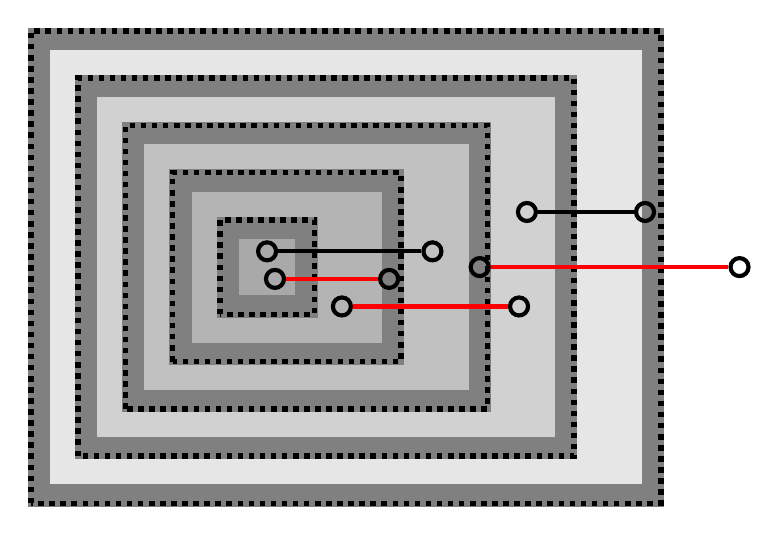
\begin{tikzpicture}[line width=1.5pt]
  \tikzstyle{every label}=[label distance=-3pt]
  \draw[biset] (-2.4,-2.4) rectangle (5.4,3.4);
  \draw[biset outer] (-2.5,-2.5) rectangle (5.5,3.5);
  \draw[biset] (-1.8,-1.8) rectangle (4.3,2.8);
  \draw[biset outer] (-1.9,-1.9) rectangle (4.4,2.9);
  \draw[biset] (-1.2,-1.2) rectangle (3.2,2.2);
  \draw[biset outer] (-1.3,-1.3) rectangle (3.3,2.3);
  \draw[biset] (-.6,-.6) rectangle (2.1,1.6);
  \draw[biset outer] (-.7,-.7) rectangle (2.2,1.7);
  \draw[biset] (0,0) rectangle (1,1);
  \draw[biset outer] (-.1,-.1) rectangle (1.1,1.1);

  \node[vertex, label=north:] (v1) at (6.5,.5){};
  \node[vertex, label={[label distance=-4pt]north west:}] (v2) at (5.3,1.2){};
  \node[vertex, label=north:] (v2n) at (3.8,1.2){};
  \node[vertex, label={[label distance=-7pt]south west:}] (v3) at (3.2,.5){};
  \node[vertex, label=south:] (v3n) at (3.7,0){};
  \node[vertex, label=north:] (v4) at (2.6,.7) {};
  \node[vertex, label=south:] (v5) at (1.45,0) {};
  \node[vertex, label={[label distance=-3pt]east:}] (v5n) at (2.05,.35) {};
  \node[vertex, label={[label distance=-7pt]north east:}] (v6) at (.5,.7) {};
  \node[vertex, label={[label distance=-5pt]west:}] (v6n) at (.6,.35) {};

  \node at (5,-2) {};
  \node at (3.9,-1.4) {};
  \node at (2.8,-.8) {};
  \node at (-.25,-.2) {};
  \node at (.13,.83) {};
  \draw[red] (v1) -- (v3);
  \draw (v2) -- (v2n);
  \draw[red] (v3n) -- (v5);
  \draw (v4) -- (v6);
  \draw[red] (v5n) -- (v6n);
 \end{tikzpicture}
 \caption{An example of  and
  with . Red edges are those chosen
 in . Areas surrounded by the dotted lines represent bisets,
 and dark gray areas represent boundaries of bisets.}
 \label{fig.deletion}
 \end{figure}

Figure~\ref{fig.deletion} illustrates an example to which the deletion
algorithm is applied.
Below, we let  denote the edge set obtained by applying
the deletion algorithm to .

\begin{lemma}\label{lem.fy}
Any core in 
is covered by at least one edge in .
The core  is covered by exactly one edge in  for
 each .
\end{lemma}
\begin{proof}
 Let .
 First, we show that  is covered by exactly one edge in 
 .
 When
 the event occurs to , the algorithm adds the edge
 
 covering  to , 
 and defines  as the witness of the edge.
  is not removed by the deletion algorithm
 unless another edge covering  remains in .
 Hence  is covered by at least one edge after applying
 the deletion algorithm.
 Let  be the minimum integer in  such that
 covers .
 By way of constructing , we have .
 Suppose that another edge 
 covers  as well.
 Then,  holds.
 The definition of  indicates that .
 However, in this case, the deletion algorithm removes
  from .
 Hence,  is covered by exactly one edge in .

 
\begin{figure}[t]
 \centering

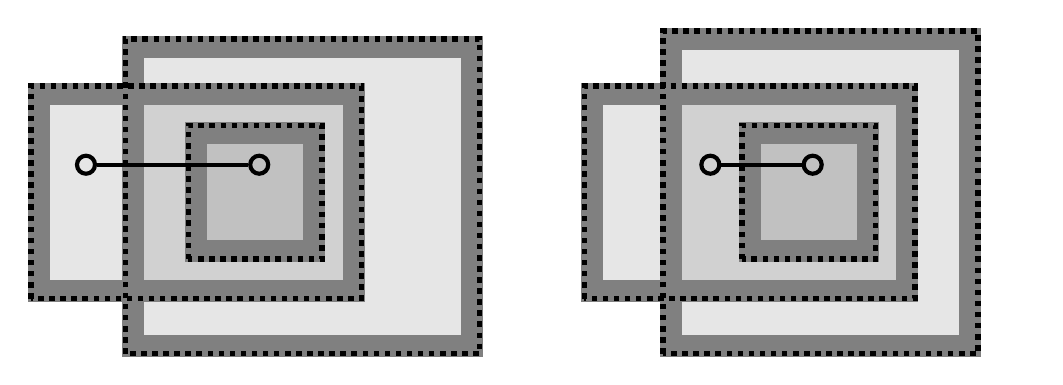
\begin{tikzpicture}[line width=1.5pt]

 \draw[biset] (1.7,-.7) rectangle +(4.3,3.8);
 \draw[biset] (.5,0) rectangle +(4,2.5);
 \draw[biset] (2.5,.5) rectangle +(1.5,1.5);
 \draw[biset outer] (1.6,-.8) rectangle +(4.5,4);
 \draw[biset outer] (.4,-.1) rectangle +(4.2,2.7);
 \draw[biset outer] (2.4,.4) rectangle +(1.7,1.7);

 \node at (.9,.4) {};
 \node at (3.5,1) {};
 \node at (5.5,-.2) {};

 \node[vertex](a) at (1.1,1.6) {};
 \node[vertex](b) at (3.3,1.6) {};
 \draw (a) -- (b);
 \node at (2.1,1.4) {};

 \begin{scope}[xshift=200pt]
 \draw[biset] (.5,0) rectangle +(4,2.5);
 \draw[biset] (1.5,-.7) rectangle +(3.8,3.9);
 \draw[biset] (2.5,.5) rectangle +(1.5,1.5);
 \draw[biset outer] (.4,-.1) rectangle +(4.2,2.7);
 \draw[biset outer] (1.4,-.8) rectangle +(4,4.1);
 \draw[biset outer] (2.4,.4) rectangle +(1.7,1.7);

 \node at (.9,.4) {};
 \node at (3.5,1) {};
 \node at (6,.5) {};

 \node[vertex](c) at (2,1.6) {};
 \node[vertex](d) at (3.3,1.6) {};
 \draw (c) -- (d);
 \node at (2.9,1.4) {};

 \end{scope}
\end{tikzpicture}

 \caption{Bisets in the proof of Lemma~\ref{lem.fy}. The left figure
illustrates the case where , and the right figure illustrates the
 case where .}
 \label{fig.lemmafy}
\end{figure}

 Let .
 We show that  is covered by at least one edge in .
  To the contrary,
 suppose that   is 
 covered by no edge in .
 Let  be a maximal core among such cores,
 and let  be the maximum integer in  such that 
 .
 By the above claim,  contains the edge
  covering .
 Since  does not cover , we have , and
  holds because .

 Suppose that .
 The left example in Figure~\ref{fig.lemmafy}
 illustrates this case.
 By the maximality of , 
  is not included by , and hence
  holds.
 Since ,
 the maximality of  indicates that
  is covered by an edge in .
 Let
  be an edge in  covering .
 Since ,  does not cover
 , implying .
  covers  or .
 If  covers , then
  is covered by two edges in , which is a contradiction.
 Hence,  covers , which is a contradiction again.

 Next, consider the case where .
 The example on the right side of Figure~\ref{fig.lemmafy} illustrates this case.
  follows from .
 Hence, , and  does not cover
 .
 By the maximality of ,  is not included by ,
 and hence .
 By Lemma~\ref{lem.afam},  was a minimal core in
 
 that was not covered by  when  was added to .
 Note that .
 Hence, an edge in  covered 
 when  was added to .
 Let  denote such an edge.
 Since  does not cover ,
 we have , implying that the witness of  is
 included by .
  is not the witness of  because .
 Hence, the witness of  is also included by .
 From this, it follows that .
 However, it indicates that  does not cover ,
 which is a contradiction.
 \end{proof}


Let  be the node that each edge in  leaves.
When , 
let  be the family of witnesses of edges in .
We apply the deletion algorithm to each
 to obtain , and define .
When ,
let  be the witness of the edge in ,
and let  be the family of  and maximal cores in
 that is not comparable with .
We apply the deletion algorithm to each core  to
obtain  and define 
when .
In the following lemmas, it will be shown that  is a spider with 
 feet and  is the head of .

\begin{lemma}\label{lem.spider1}
 When ,
 the edge set 
  is a spider with only one foot, and its head is .
\end{lemma}
\begin{proof}
 Let  be the witness of the edge in 
 and  be the min-core included by .
 We prove that  is a spider and its foot is .
 Lemma~\ref{lem.fy} indicates that all cores in  are
 covered by .
 Hence, it suffices to show that
 each core  with  is covered by
 .
 Suppose that  is covered by no edge in .
 Let  be the minimal core among such cores.
 There exists an edge  that covers .
 Let  be the witness of , and let  and
 , without loss of generality. If ,
 then  remains in .
 Hence .
  is either incomparable with
  or is included by .
 If more than one edge in  cover  and one of them
 gives  incomparable with ,
 then we choose such an edge as .

 \begin{figure}[th]
  \centering
 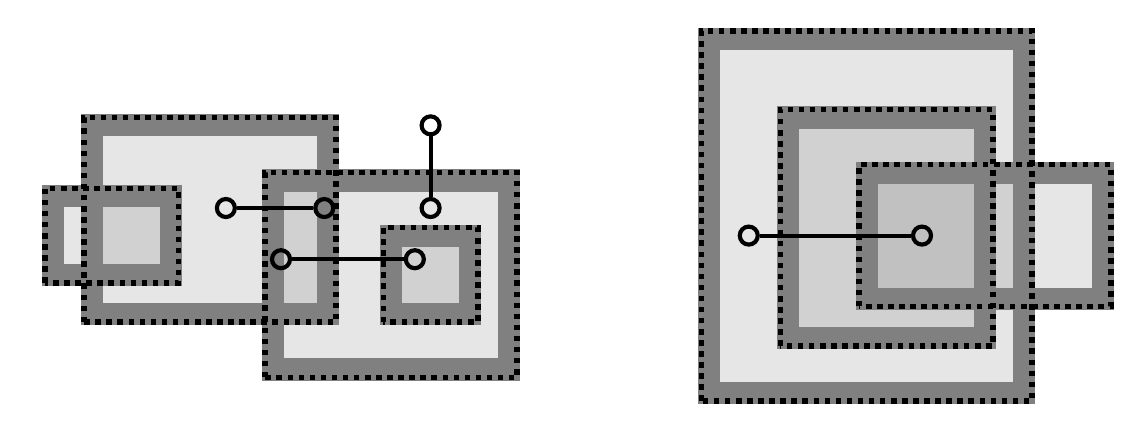
\begin{tikzpicture}[line width=1.5pt]
  \draw[biset] (-1,-.5) rectangle (.5,.5);
  \draw[biset] (-.5,-1) rectangle +(3,2.4);
  \node at (-1.2,-.9) {};
  \node at (1.1,-.6) {};

  \draw[biset] (1.8,-1.7) rectangle +(3,2.4);
  \draw[biset] (3.3,-1) rectangle +(1,1);
  \node at (3.9,-.6) {};
  \node at (5.3,-1.4) {};

  \draw[biset outer] (-1.1,-.6) rectangle (.6,.6);
  \draw[biset outer] (-.6,-1.1) rectangle +(3.2,2.6);
  \draw[biset outer] (1.7,-1.8) rectangle +(3.2,2.6);
  \draw[biset outer] (3.2,-1.1) rectangle +(1.2,1.2);

  \node[vertex] (a) at (3.6,-.3){};
  \node[vertex] (b) at (1.9,-.3){};
  \draw (a) -- (b);
  \node at (2.9,-.1) {};

  \node[vertex] (c) at (3.8,.35){};
  \node[vertex] (d) at (3.8,1.4){};
  \draw (c) -- (d);
  \node at (4,1.1) {};

  \node[vertex] (e) at (1.2,.35){};
  \node[vertex] (f) at (2.45,.35){};
  \draw (e) -- (f);
  \node at (2.2,.1) {};

  \begin{scope}[xshift = 280pt]
   \draw[biset] (-2.5,-2) rectangle (1.5,2.5);
   \draw[biset] (-1.5,-1.3) rectangle (1,1.5);
   \draw[biset] (-.5,-.8) rectangle +(3,1.6);

   \draw[biset outer] (-2.6,-2.1) rectangle (1.6,2.6);
   \draw[biset outer] (-1.6,-1.4) rectangle (1.1,1.6);
   \draw[biset outer] (-.6,-.9) rectangle +(3.2,1.8);

   \node at (-2.1,2.1) {};
   \node at (-1,1.1) {};
   \node at (2.1,-.3) {};
   
  \node[vertex] (a) at (-2,0){};
  \node[vertex] (b) at (.2,0){};
  \draw (a) -- (b);
  \node at (-1,-.2) {};
  \end{scope}
 \end{tikzpicture}
  \caption{Bisets in the proof of Lemma~\ref{lem.spider1}. The left
  figure illustrates the case where  is incomparable with
  , and
  the right illustrates the case where  is included by .}
  \label{fig.spider1}
 \end{figure}

 Suppose that  is incomparable with .
 The left example in Figure~\ref{fig.spider1} illustrates this case.
 Let  be the min-core included by ,
 and let  be the minimal core in  with
 .
 Note that , and
  and  are incomparable.
 Then,  holds, and 
 it is covered by some edge  by Lemma~\ref{lem.fy}.
 Since  does not cover , it has one end-node in  and the other in .
 On the other hand, .
 The minimality of  indicates that 
 is covered by some edge .
 Since  does not cover ,
 it has one end-node in  and the other in .
 These imply that , and both  and  cover .
 If , then this is a contradiction because
 any core in 
 is covered by exactly one edge in  by Lemma~\ref{lem.fy}.
 Otherwise, .
 Even in this case, there is a contradiction because each core in  is covered by no edge in .

 Suppose that  is included by .
  holds.
 Moreover,  holds
 because  includes , 
 and  holds
 because  is included by .
  is covered by some edge .
 The witness of  is incomparable with 
 since otherwise, .
  covers  or .
 If  covers ,
 then  is chosen instead of , and this case is categorized into
 the previous one where  is incomparable with .
 Hence,  covers . Then,
 Lemmas~\ref{lem.uncrossable}~(iii) and \ref{lem.afam} indicate that
 all cores comparable with the witness of
  
 are covered by  before  is added to ,
 which is
 a contradiction.
\end{proof}

 \begin{lemma}\label{lem.spider2}
 When ,
  the edge set 
  is a spider with  feet, and  is its head.
\end{lemma}
\begin{proof}
 Let  be the set of witnesses of
 the edges in .
 Let  be the min-core included by ,
 and let  denote 
 for each .
 Lemma~\ref{lem.fy} shows that  covers 
 for each .
 Hence it suffices to prove that 
  for each
  with .
 Suppose that  and  share an
 end-node  with .
 
 Suppose that  was added to 
 before .
 Let 
 be the witness of , and  be the core 
 that was added to  when  was removed from .
 Note that , and
  does not cover  but .
 Hence, ,
 and the other end-node of  is in .
 If , then
  covers all cores including 
 since they are strongly disjoint with .
 Hence, Case (b) occurred when  was added to , 
 and  must be  in this case.
 Even if , 
  and  are added to  because of the directed edges leaving .
 This means that
 Case (b) occurred when  was added to ,
 and  holds.
\end{proof}


\begin{lemma}\label{lem.spider-lp}
 There exists  such that  is
 activated by , and .
\end{lemma}
\begin{proof}
 Recall that each edge in  is undirected, but it has a unique
 direction in which it enters the inner-part of its witness.
 Hence, we regard the edges in  as directed edges in this proof.
 For each ,
 there exists 
 such that 
 \eqref{dual-c3'} is tight for 
  and  is tight for .
 We can activate  by setting  to a value of at least  and
  to a value of at least .
 When  is added to ,  assigns  to  and  to .
 If a node has incident edges in ,
 we set the weight of the node to the maximum value assigned from the
 incident edges in .
 If a node has no incident edge in , then its weight is set to .
 Let  be the time when the algorithm was completed.
 Below, we prove that the total weight assigned from edges in 
 is at most  where we do not count
 the weight assigned to the head  of  multiple times.
  Since , this proves
 the lemma.

 Let  be a foot of  and
  be the set of edges in  that cover .
 Let .   assigns 
 to   and  to .
 Moreover,

 holds because \eqref{dual-c3'} is tight for ,
 and 

 holds because \eqref{dual-c3} is tight for . 
 Let  denote the time when  \eqref{dual-c3'} became tight for .

 We first consider the case where .
 Let us prove that the right-hand side of \eqref{eq.je} is contributed
 by cores covered by . 
 Suppose that  holds for some  with
 . 
 Then there exists an edge
  that covers , and
 \eqref{dual-c3} was tight for some 
 with 
 at time .
  If ,
 then
 this means that Case (b) occurred when  was added to .
 Since this contradicts ,
 we have .
 If  includes the witness of ,
 then  covers  because .
 Hence,
  is included by the
 witness of . However, in this case, 
  is not added to  by the algorithm.
 Hence  covers .

 The right-hand side of \eqref{eq.je'} is also contributed by
 cores covered by .
 To see this, suppose that 
 holds for some  with .
 If  does not cover ,
 then  holds, implying that  was already in  when  entered
 .
 In other words,  enters  after time .
 However, \eqref{dual-c3} was tight for  at time .
 Therefore,  does not hold unless  covers
 . Note that this is the case even when .

 When ,  assigns  to  but 
 more than one edge leaving  in  may assign the same weight to .
 By the same discussion as above, 
 if a core  with  satisfies
 ,
 then  contains an edge that leaves  and covers .
 Hence, we here count only  as the weight assigned from  to .
 A core  contributing to this value is covered by
  according to the discussion above.
 Then the total weight assigned from edges in  is exactly
 
 Lemma~\ref{lem.fy} tells that each  is covered by exactly one edge in .
 Hence the right-hand side of the above equality is equal to .
 Since two cores in  do not belong to  simultaneously, 
 this does not exceed .
 Since  has  feet, it implies that 
 the total weight is at most .
 \end{proof}

 Theorem~\ref{thm.spideralgorithm} follows from
 Lemmas~\ref{lem.spider1}, \ref{lem.spider2},
 and \ref{lem.spider-lp}.
 


\section{Potential function on uncrossable biset families}
\label{sec.potential}

In this section,  is an uncrossable family of bisets
and  stands for .

For analyzing the greedy algorithm of choosing spiders repeatedly, we need a potential function that
measures the progress of the algorithm. Nutov~\cite{Nutov12uncrossable} used  as a
potential. He claimed that this potential gives -approximation  because
 holds for each uncrossable biset family  and
each spider  of . However, there is a case with  as
follows. Let , and suppose that 
 for each ,  and  are strongly disjoint for
each  with , and a node  is in  for
each .  is strongly laminar, and hence uncrossable. Note that
, and hence . If the head of a
spider  is  and its feet are  (i.e., ), then
 holds, and hence . Therefore,
.

Vakilian~\cite{Vakilian13} showed that such an inconvenient situation does not appear if  arises from the
node-weighted SNDP. To explain this more precisely, let  be the graph to be augmented in an
instance of the prize-collecting augmentation problem. Recall that the problem requires to add edges in an edge set  to . If this instance is obtained by the reduction from the
node-weighted SNDP in Theorem~\ref{thm.augmentation}, then  is the subset of  induced by some node set 
, and each biset  that requires to be covered satisfies .
Moreover, a spider is not chosen if its head is in , 
and therefore the heads of chosen spiders are not included by the neighbor
of any biset. This means that each spider  achieves  for  arising
from the node-weighted SNDP. However this is not the case for all uncrossable biset families, including those arising from 
the PCNAP because  may not be an induced subgraph in general.

Because of this, using  as a potential function gives no desired
approximation guarantee for general uncrossable biset families. Hence, we introduce a new potential function in this section. For a family
 of cores and core ,  let 
denote the set of nodes  such that  there exists another core  with . We define the potential
 of a core  as . The
potential  of  is defined as 
.



\begin{lemma}\label{lem.neighbor}
 Let ,  be an edge set, and  be the
 min-core in  
 such that  where  possibly holds.
 Let  be a node with
 ,
 and  be a min-core in  with .
 Then,  covers all cores in . If there exists a min-core in
  that includes , then it is .
\end{lemma}
\begin{proof}
 Since ,
  is either in  or .
 Suppose it is the former case (i.e., ). Then,  
 because  and  are not strongly disjoint in this case,
 and 
 contradicts Lemma~\ref{lem.uncrossable}~(iii).
 Moreover,  is
 included by  
 since, otherwise, they must be strongly disjoint, contradicting the
 existence of .
 This means that all cores
 in  are covered by .

 Suppose it is the latter case (i.e., ). 
 Let  be a min-core in  that includes , and
 assume that it is distinct from .
 Since , no min-core
 in  contains  in its neighbor.
 Hence .
 However, this means that 
  and  are not strongly disjoint, which contradicts
 Lemma~\ref{lem.uncrossable}~(iii).
 This implies that  covers  since,
 if  contains a core not covered by , then
 the minimal core among such cores is a min-core in  distinct
 from .
\end{proof}


\begin{lemma}\label{lem.newcore}
 Let  be an edge set and .
 Then, exactly one of the following holds\/{\rm :}
\begin{itemize}
 \item  includes at least two min-cores in ,
       and all cores of  including these min-cores are covered by
       \/.
 \item  is a core of  that includes 
       a min-core in .
\end{itemize}
\end{lemma}
\begin{proof}
 Since , there exist min-cores in 
 included by . Suppose that the number of such min-cores is
 one, and we call the min-core by . Then,
  is a core of .
 Since ,  is covered by , and hence,
 .
 If the number of such min-cores is at least two, 
 then the cores of  including such min-cores are covered by 
 because  is minimal in .
\end{proof}

\begin{lemma}\label{lem.potentialdecrease}
 Let  be a spider for . If , then 
 .
 Otherwise, .
\end{lemma}
\begin{proof}
 Let  denote the number of min-cores
 
 such that  covers all bisets in , and let  denote the
 number of min-cores  
 such that  covers  but not all bisets in .
 Note that  holds.
 If  is a min-core counted in ,
 then there exists a unique min-core  that
 includes . Let  denote the set of pairs of such  and .

 Let  be a min-core counted in .
 If a core of  includes , then
 the core includes at least two min-cores in .
 Let  be the set of such  that
 is included by a min-core in , 
 and let  be the set of such 
 that 
 is included by no min-core of  (although it may be included by a core in ).
 Note that .

 By Lemma~\ref{lem.newcore},
 each min-core in   
 includes at least two members of  
 or belongs to  defined by a min-core 
  covered by .
 Hence
 .
 From this, it follows that 
 
 
 Recall that
  is defined as ,
 and 
  is defined as 
 .
 The first term of 
 is larger than that of  by .
 A min-core  either includes at least two members of
  or belongs to  defined by a
 min-core  (i.e., ).
 There are at most  min-cores of the former type, and hence
 the sum of their potentials is at most .
 Let  belong to the latter type. 
 Note that
 
 If there exists ,
 then there exists  counted in  such that , and  by Lemma~\ref{lem.neighbor}. 
 We make  give one token to .
 Then,  obtains  tokens. 
 Note that only  contains  in its
 outer-part among all min-cores in ;
 If , then
 it is implied by the strong disjointness of min-cores, and 
 if , then it is implied by .
 Hence, each  releases at most
 one token for each node .
Therefore, the total number of tokens is at most , and
hence,

 Summing up, 



 If , then , and hence  by \eqref{eq.potential-lowerbound}. Since potentials are integers, this means that 
 .
 Suppose that . 
  Consider the case where the head of  is included by the inner-part
 of some min-core .
 If a foot  of  is strongly disjoint from , 
 then  is covered by , and hence  is counted in .
 If  includes at least two feet of , then all cores of 
 including these feet are covered by . Therefore,
 , and hence
  by \eqref{eq.potential-lowerbound}.

 In the remaining case,  and 
 no min-core in  contains
the head  of  in its inner-part.
By definition of spiders, each foot  is covered by .
 Hence  is counted in  or .
 If , then we are done. Hence, suppose that
 .  feet of  are counted in .
 Let  be a foot of  that is counted in .
 Then, there exists  with
  and .
 Since  contains at least two such ,
 we have .
 Therefore,

 and \eqref{eq.potential-lowerbound} implies that
 .
 \end{proof}

\begin{theorem}\label{thm.potential-spider}
 Let  be an uncrossable family of bisets.
 There exist ,
 a spider  activated by ,
 and a strongly laminar family  of cores of 
 such that 
 
\end{theorem}
\begin{proof}
 Theorem~\ref{thm.spideralgorithm} shows that
 there exist , 
 a spider  activated by , and a strongly laminar family  of cores
 such that
 
 Since , we have



 If , then  by
 Lemma~\ref{lem.potentialdecrease}, and hence, the required inequality
 follows from \eqref{eq.potential-1}.
 Otherwise,
  by
 Lemma~\ref{lem.potentialdecrease}, and hence,

 where the first inequality follows from .
Combining with \eqref{eq.potential-1}, this gives

\end{proof}

Our algorithm presented in Section~\ref{sec.primal-dual}
computes the node weights  and spider  claimed by
Theorem~\ref{thm.potential-spider} in polynomial time. 
Alternatively, one can use the 
simpler algorithm in~\cite{Nutov13activation}, which approximates 
within a factor of .


\section{Algorithm}
\label{sec.algorithm}

We first present our main theorem.

\begin{theorem}\label{thm.main}
 Suppose that  is a biset family such that  is
 uncrossable for each .
 Let 
 and .
 The prize-collecting biset covering problem with  admits an -approximation algorithm.
\end{theorem}
\begin{proof}
 Let  be an optimal solution for .
 We first compute .
 We eliminate all demand pairs  such that ,
 and eliminate each biset that separates no remaining demand pair from .
 Let  be the biset family obtained after this operations.
  holds
 because  is feasible to .

 Applying Theorem~\ref{thm.potential-spider} to ,
 we obtain ,  and  
 such that
 ,
and the right-hand side is at most 
 by Lemma~\ref{lem.corelpvslp}.
 If , then
 we apply
 Theorem~\ref{thm.potential-spider} to .
 Let  and  be the obtained node weights and spider, respectively.
 We add edges in  to ,
 increase the weight  by  for each .
 We repeat this until  becomes 0.
 By a standard argument of the greedy algorithm for the set cover problem,
 we have 
 when the above procedure is completed.
 Since ,
 it implies that .

The penalty of  is at most 
 because  covers all bisets separating each demand pair 
 with , and .
 .
 Therefore the objective value of  is 
 times .
 Lemma~\ref{lem.relaxation} shows that  is at most the
 optimal value of the prize-collecting biset covering problem.
\end{proof}


\begin{corollary}\label{cor.edge-element}
 Let .
 The edge-connectivity PCNAP admits an -approximation
 algorithm, and
 the element-connectivity PCNAP admits an -approximation
 algorithm.
 \end{corollary}
\begin{proof}
 is an uncrossable family of bisets with .
 Hence, Theorems~\ref{thm.augmentation} and \ref{thm.main} give
 an -approximation algorithm for the edge-connectivity PCNAP.
 is an uncrossable family of bisets
 with .
 Hence, Theorems~\ref{thm.augmentation} and \ref{thm.main} give
 an -approximation algorithm for the element-connectivity PCNAP.
\end{proof}

We note that 
. Hence, the above corollary gives
an -approximation algorithm for the edge-connectivity
PCNAP,
and an -approximation algorithm for the element-connectivity
PCNAP.

The next corollary provides approximation algorithms for the
node-connectivity requirements.
Since it is reasonable to suppose  for the node-connectivity
requirements,
the next corollary does not have  in contrast with Corollary~\ref{cor.edge-element}.

\begin{corollary}\label{cor.node}
\begin{itemize}
 \item[\rm (i)] The node-connectivity PCNAP admits an
	      -approximation randomized algorithm.
 \item[\rm (ii)] The rooted node-connectivity PCNAP admits an
	      -approximation algorithm.
 \item[\rm (iii)] The subset node-connectivity PCNAP admits an
	      -approximation algorithm.
\end{itemize}
 \end{corollary}
\begin{proof}
 Theorem~\ref{thm.augmentation}
 reduces the node-connectivity PCNAP
 to the prize-collecting biset covering problem with the biset family
  by paying factor .
 Chuzhoy and Khanna~\cite{ChuzhoyK12} presented a randomized algorithm
 for decomposing an instance of the node-connectivity SNDP into 
  instances of the element-connectivity SNDP such that
 the union of solutions for the  instances is 
 feasible to the original instance.
 This algorithm can be applied for
 computing   
 uncrossable subfamilies of 
 such that an edge set covering the union of the subfamilies
 covers .
 By Theorem~\ref{thm.main}, 
 we compute -approximate solutions for
 instances of 
 the prize-collecting biset covering problem 
 with the subfamilies. We then return the union of the obtained solutions.
 This achieves
 -approximation for the original instance
 of the node-connectivity PCNAP.

 For the rooted node-connectivity PCNAP, 
 we replace the decomposition result due to Chuzhoy and Khanna~\cite{ChuzhoyK12} by
 the one due to Nutov~\cite{Nutov12uncrossable}, which proved
 that 
 can be decomposed into  uncrossable subfamilies.
 This achieves -approximation for the rooted
 node-connectivity PCNAP.

 Strictly speaking,
 Theorem~\ref{thm.augmentation} cannot be applied to the subset
 node-connectivity PCNAP because it is not a special case of the PCNAP, 
 but we can similarly prove that the same claim holds for
 the subset node-connectivity PCNAP.
  Using a decomposition result in Nutov~\cite{Nutov12subset},
 the augmentation problem obtained by the reduction 
 can be decomposed into
 one instance with the rooted node-connectivity requirements and  instances  with single demand pairs.
 The former instance can be approximated within a factor of 
 as above.
 Each of the latter instances admits a constant factor approximation
 using the algorithm presented in \cite{Nutov13activation}.
 These give -approximation for the original augmentation unless . 
 When  (including the case with ), 
 the augmentation problem can be decomposed into  instances
 with single demand pairs, resulting in an -approximation for
 the augmentation problem.
 Recall that we pay factor  for reducing PCNAP to the
 prize-collecting augmentation problem.
 Therefore, we have an -approximation algorithm for the
 subset node-connectivity PCNAP.
\end{proof}

Note that  in Corollary~\ref{cor.node}.

\section{Conclusion}\label{sec.conclusion}

We have presented approximation algorithms for PCNAP.
Our algorithms are built on new formulations of LP relaxations, the primal-dual algorithm for computing spiders, and the potential
function for analyzing the greedy spider cover algorithm.

Our algorithms must solve the LP relaxation in order to decide which demand
pairs should be satisfied by solutions. In contrast, several primal-dual algorithms such as
those in \cite{BateniHL13,Konemann13CoRR} can manage this without solving LP
by generic LP solvers.
In other words, these algorithms are combinatorial.
We believe that it is challenging to design combinatorial algorithms for PCNAP.


\section*{Acknowledgements}

This work was supported by
JSPS KAKENHI Grant Number 25730008 in part.
The author thanks Zeev Nutov for sharing information on his paper \cite{Nutov12uncrossable}.



\begin{thebibliography}{10}

\bibitem{BateniHL13}
M.~Bateni, M.~Hajiaghayi, and V.~Liaghat.
\newblock Improved approximation algorithms for (budgeted) node-weighted
  {S}teiner problems.
\newblock In {\em ICALP (1)}, vol. 7965 of {\em Lecture Notes in Computer
  Science}, pages 81--92, 2013.

\bibitem{BienstockGSW93}
D.~Bienstock, M.~X. Goemans, D.~Simchi-Levi, and D.~P. Williamson.
\newblock A note on the prize collecting traveling salesman problem.
\newblock {\em Mathematical Programming}, 59:413--420, 1993.

\bibitem{ChekuriEV12}
C.~Chekuri, A.~Ene, and A.~Vakilian.
\newblock Prize-collecting survivable network design in node-weighted graphs.
\newblock In {\em APPROX-RANDOM}, vol. 7408 of {\em Lecture Notes in Computer
  Science}, pages 98--109, 2012.

\bibitem{ChuzhoyK12}
J.~Chuzhoy and S.~Khanna.
\newblock An {O}-approximation algorithm for vertex-connectivity
  survivable network design.
\newblock {\em Theory of Computing}, 8(1):401--413, 2012.

\bibitem{FleischerJW06}
L.~Fleischer, K.~Jain, and D.~P. Williamson.
\newblock Iterative rounding 2-approximation algorithms for minimum-cost vertex
  connectivity problems.
\newblock {\em Journal of Computer and System Sciences}, 72(5):838--867, 2006.

\bibitem{Fukunaga14}
T.~Fukunaga.
\newblock Covering problems in edge- and node-weighted graphs.
\newblock In {\em SWAT}, vol. 8503 of {\em Lecture Notes in Computer Science},
  pages 217--228, 2014.

\bibitem{HajiaghayiKKN12}
M.~T. Hajiaghayi, R.~Khandekar, G.~Kortsarz, and Z.~Nutov.
\newblock Prize-collecting steiner network problems.
\newblock {\em {ACM} Transactions on Algorithms}, 9(1):2, 2012.

\bibitem{Jain01}
K.~Jain.
\newblock A factor 2 approximation algorithm for the generalized {S}teiner
  network problem.
\newblock {\em Combinatorica}, 21(1):39--60, 2001.

\bibitem{KleinR95}
P.~N. Klein and R.~Ravi.
\newblock A nearly best-possible approximation algorithm for node-weighted
  {S}teiner trees.
\newblock {\em Journal of Algorithms}, 19(1):104--115, 1995.

\bibitem{Konemann13CoRR}
J.~K{\"o}nemann, S.~S. Sadeghabad, and L.~Sanit{\`a}.
\newblock An {LMP} -approximation algorithm for node weighted
  prize collecting {S}teiner tree.
\newblock In {\em FOCS}, pages 568--577, 2013.

\bibitem{MossR07}
A.~Moss and Y.~Rabani.
\newblock Approximation algorithms for constrained node weighted {S}teiner tree
  problems.
\newblock {\em {SIAM} Journal on Computing}, 37(2):460--481, 2007.

\bibitem{Nutov10node-weights}
Z.~Nutov.
\newblock Approximating {S}teiner networks with node-weights.
\newblock {\em {SIAM} Journal on Computing}, 39(7):3001--3022, 2010.

\bibitem{Nutov12uncrossable}
Z.~Nutov.
\newblock Approximating minimum-cost connectivity problems via uncrossable
  bifamilies.
\newblock {\em {ACM} Transactions on Algorithms}, 9(1):1, 2012.

\bibitem{Nutov12subset}
Z.~Nutov.
\newblock Approximating subset -connectivity problems.
\newblock {\em Journal of Discrete Algorithms}, 17:51--59, 2012.

\bibitem{Nutov13activation}
Z.~Nutov.
\newblock Survivable network activation problems.
\newblock {\em Theoretical Computer Science}, 514:105--115, 2013.

\bibitem{Panigrahi11wireless}
D.~Panigrahi.
\newblock Survivable network design problems in wireless networks.
\newblock In {\em SODA}, pages 1014--1027, 2011.

\bibitem{Vakilian13}
A.~Vakilian.
\newblock Node-weighted prize-collecting survivable network design problems.
\newblock Master's thesis, University of Illinois at Urbana-Champaign, 2013.

\end{thebibliography}
 \end{document}
